\chapter{Related Work}
\label{sec:related}

%----Retinex理論の説明---- %
\section{Retinex Theory} \label{sec:retinex}
The Retinex theory \cite{retinex} is a color perception model based on human visual system. The model decomposes an observed image into the reflectance and illumination as follows:
\begin{equation}
S = R \circ I,\label{eq:retinex}
\end{equation}
where $S$ is an observed image, $R$ and $I$ represent the reflectance and the illumination, respectively. The operator $\circ$ denotes the element-wise multiplication. As shown in Fig. \ref{fig:retinex}, the reflectance represents the intrinsic characteristics of the object and contains rich textures detail. On the contrary, the illumination represents the extrinsic property and contains the structure information with texture-less.

%----Retinex理論のイメージ図---- %
\begin{figure}[tb]
	\begin{minipage}[b]{0.32\hsize}
		\centering
		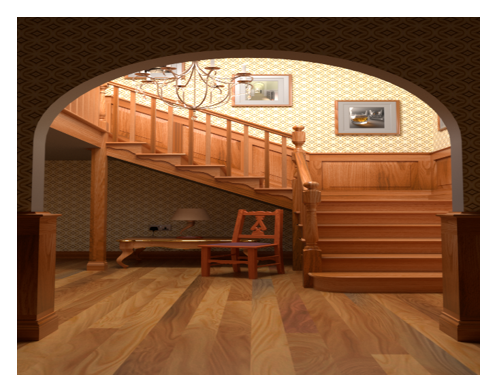
\includegraphics[height=0.75\hsize]{images/retinex/input.eps}
		\subcaption{Observed image $S$} \label{fig:reinex/input}
	\end{minipage}
	\begin{minipage}[b]{0.32\hsize}
		\centering
		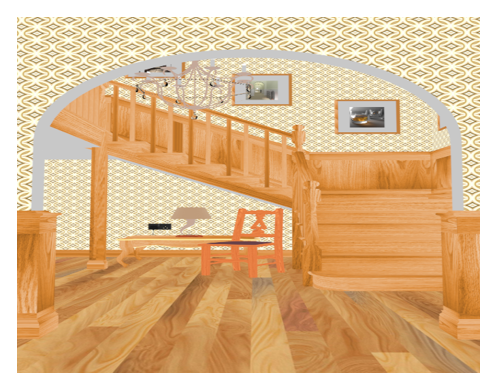
\includegraphics[height=0.75\hsize]{images/retinex/reflectance.eps}
		\subcaption{Reflectance $R$} \label{fig:retinex/reflectance}
	\end{minipage}
	\begin{minipage}[b]{0.32\hsize}
		\centering
		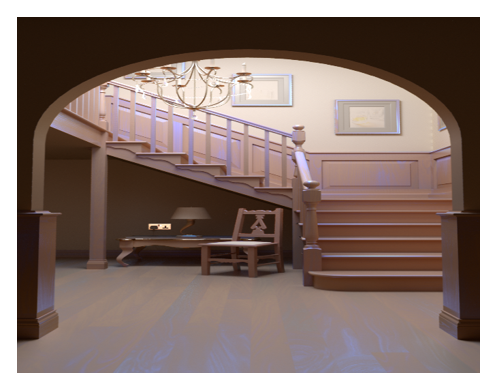
\includegraphics[height=0.75\hsize]{images/retinex/illumination.eps}
		\subcaption{Illumination $I$} \label{fig:retinex/illumination}
	\end{minipage}
\caption{The images represent Retinex theory \cite{arpr}.}
\label{fig:retinex}
\end{figure}

The conventional Retinex-based enhancement methods such as \cite{ssr}, \cite{msr} are defined as
\begin{equation}
\log{R} = \log{S} - \log{[G \ast S]}, \label{eq:log_retinex}
\end{equation}
where $\ast$ represents the convolution operator, $G$ is the Gaussian low-pass filter. This method assumes that illumination can be estimated by the Gaussian low-pass filtered version of an observed image. Moreover, the reflectance is computed by subtracting the estimated illumination from an observed image. However, this method generates the halo effect around the edges of object according to the size of the Gaussian low-pass filter. In addition, as shown in Fig. \ref{fig:msr}, this method cause over-enhancement and much noise in the estimated reflectance. 

\begin{figure}
\begin{minipage}[b]{0.5\hsize}
		\centering
		\includegraphics[height=0.6\hsize]{images/msr/input.eps}
		\subcaption{Observed image $S$} \label{fig:msr/input}
	\end{minipage}
	\begin{minipage}[b]{0.5\hsize}
		\centering
		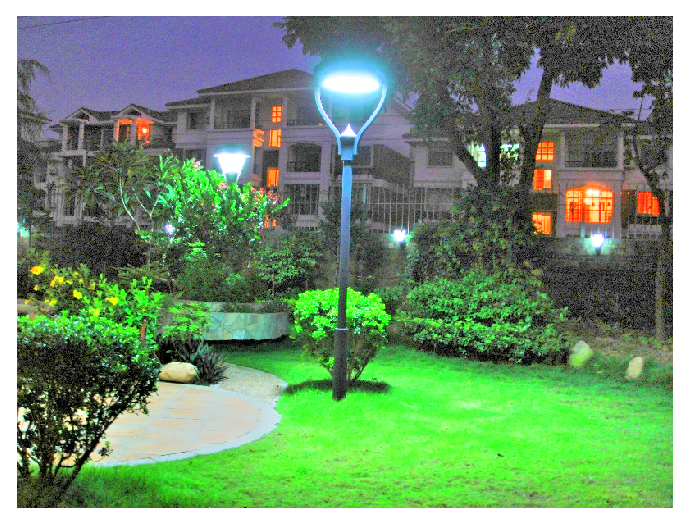
\includegraphics[height=0.6\hsize]{images/msr/reflectance.eps}
		\subcaption{Reflectance $R$} \label{fig:msr/reflectance}
	\end{minipage}
\caption{The images represent the result of the conventional Retinex-based enhancement method \cite{msr}.}
\label{fig:msr}
\end{figure}

%----Variational Retinex Modelの説明---- %
\section{Variational Retinex Model} \label{sec:variational_retinex}
Various researches have proposed energy minimization problems based on Retinex in order to efficiently estimate reflectance and illumination. These methods estimate reflectance and illumination by setting the constraint terms which consider the characteristics for their component. Thus, it is important for these methods to adopt the appropriate constraints for their component in order to deal with halo effect, over-enhancement, and noise amplification. These methods usually adopt the $L_{1}$ and $L_{2}$ norm regularization to the constraint terms. To give an example, Fu \cite{srie} proposed the minimizing optimization problem derived as
\begin{equation}
\begin{split}
& E(I, R) = \argmin_{R, I} \|R \circ I - S\|_{2}^{2} + \alpha\|\nabla{I}\|_{2}^{2} + \beta\|\nabla{R}\|_{1} + \gamma\|I - I_{0}\|_{2}^{2} \\
& s.t. \ \ S \leqq I, \label{eq:srie_equation}
\end{split}
\end{equation}
where $\alpha$, $\beta$, $\gamma$ are three positive parameters, and $I_{0}$ is the enhanced illumination using gamma correction.
The first term $\|R \circ I - S\|_{2}^{2}$, which corresponds to L2 data fidelity, is to minimize the distance between the estimated ($R\circ{I}$) and an observed image $S$. The second term $\|\nabla{I}\|_{2}^{2} $ enforces spatially smoothness on the illumination $I$. The third term $\|\nabla{R}\|_{1}$, which corresponds to TV reflectance sparsity, enforces piece-wise continuous on the reflectance $R$. The last term $\|I-I_{0}\|_{2}^{2}$, which penalizes the brightness of illumination component, is used to avoid a scaling problem. \par
This method demonstrated the linear domain model is better than the log-transformed domain model in preserving naturalness. As shown in Fig. \ref{fig:variational/srie}, this method can suppress the over-enhancement in the estimated reflectance thanks to the third term which minimizes the difference between $I$ and $I_{0}$. Moreover, since this method imposes $L_{1}$ norm regularization on the reflectance, the estimated reflectance can suppress noise amplification.

%----SRIEの図---- %
\begin{figure}[htbp]
	\begin{minipage}[b]{0.5\hsize}
		\centering
		\includegraphics[width=62.5mm]{images/variational/input.eps}
		\subcaption{Observed image $S$} \label{fig:variational/input}
	\end{minipage}
	\begin{minipage}[b]{0.5\hsize}
		\centering
		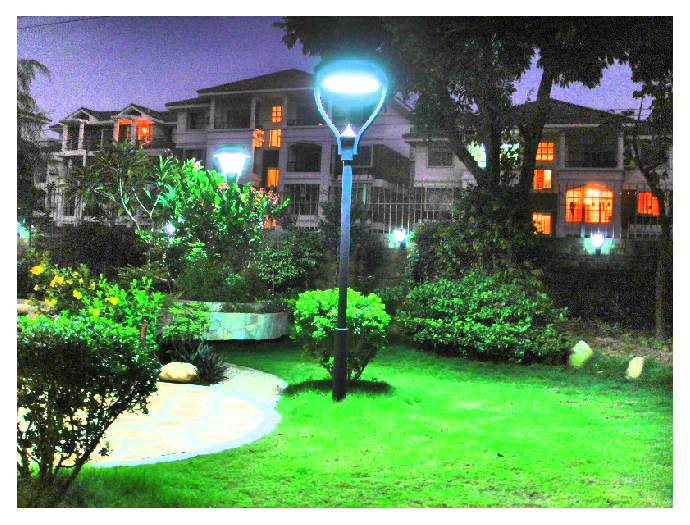
\includegraphics[width=62.5mm]{images/variational/reflectance.eps}
		\subcaption{Reflectance $R$} \label{fig:variational/reflectance}
	\end{minipage}
	\begin{minipage}[b]{0.5\hsize}
		\centering
		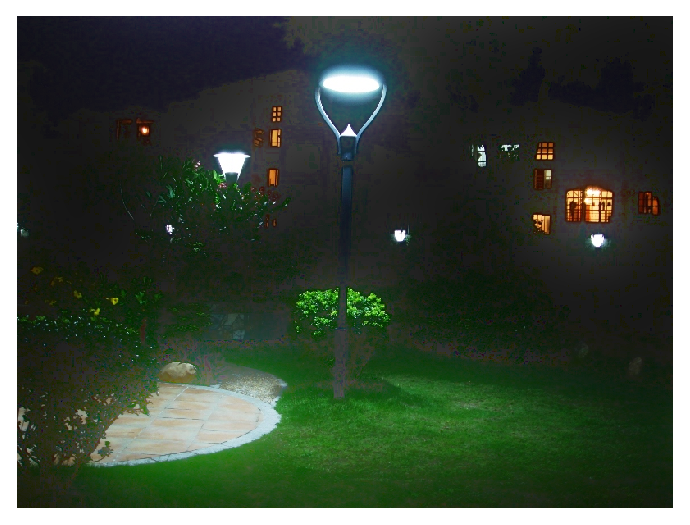
\includegraphics[width=62.5mm]{images/variational/illumination.eps}
		\subcaption{Illumination $I$} \label{fig:variational/illumination}
	\end{minipage}
	\begin{minipage}[b]{0.5\hsize}
		\centering
		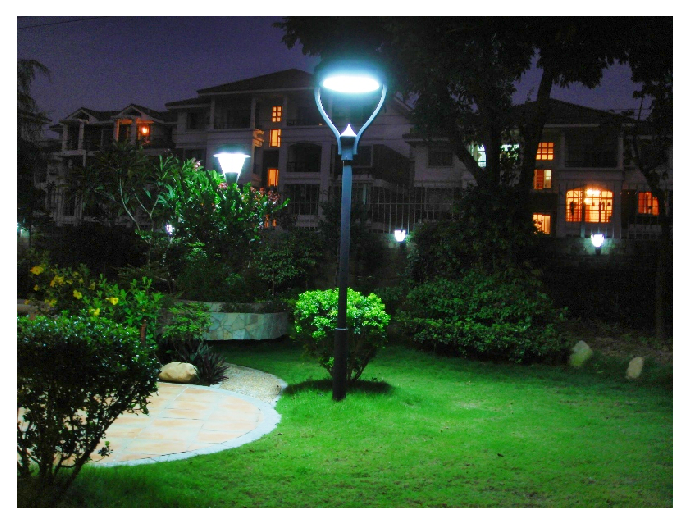
\includegraphics[width=62.5mm]{images/variational/output.eps}
		\subcaption{Enhanced image $\hat{S}$} \label{fig:variational/output}
	\end{minipage}
	\caption{The images represent the result of SRIE \cite{srie}.}
	\label{fig:variational/srie}
\end{figure}

%----Edge Preserving Filterの説明---- %
\section{Local Variation Deviation} \label{sec:lvd}
In this section, the review centers on the edge/structure preserving image smoothing and the joint intrinsic-extrinsic prior model (JieP), which proposed by Cai \cite{jiep} and adopted the image smoothing function as the constraint term on the illumination in (\ref{eq:srie_equation}). 
%The illumination is piece-wisely smooth component, which can be decomposed by a edge preserving smoothing.
\par
In statics, the standard deviation represents a measure to quantify the consistency of a set of data. The local variation deviation (LVD) is used to identify different type of the variation with its statistical property. By using the feature in the image analysis, the local variation deviation can surprisingly distinguish between texture and structure, since texture component has the feature of weak correlation and structure component has the feature of strong correlation. \par
The $\mathcal{R}_{d}$ denotes the relative LVD extracted from $I$:

\begin{equation}
\mathcal{R}_{d} = \left |\frac{\nabla_{d}{I}}{\frac{1}{\Omega}\Sigma_{\Omega}\nabla_{d}{I}+\epsilon} \right| ,
\label{eq:lvd}
\end{equation} 
where $\nabla_{d}$ is the horizontal/vertical ($d \in {h, v}$) gradient operator, $\Omega$ is the local patch size $(r \times r)$, and $\epsilon$ is a small number to avoid division by zero. 
The edge/structure preserving smoothing property of the LVD can be explained intuitively as following.
(In the following, the variable of the mean local variation means $\bar{\nabla{I}}= \frac{1}{|\Omega|} \Sigma_{\Omega}\nabla{I}$):

\begin{itemize}
\item Case1: \textbf{Flat.} If the value of the patch $I$ is almost constant, $\nabla{I} \approx 0$ and $\bar{\nabla{I}} \approx 0$ $\rightarrow$ $\bar{\mathcal{R}} \approx 0$. 
\item Case2: \textbf{Texture.} If the value of the patch $I$ changes frequently, $\nabla{I} $ varies more rapidly than $\bar{\nabla{I}}$ $\rightarrow$ $\bar{\mathcal{R}}$ $\gg 1$.
\item Case3: \textbf{Structure.} If the value of the patch $I$ changes in accordance with structure, the deviation of $\nabla{I}$ fluctuates small $\rightarrow$ $\bar{\mathcal{R}}$ $\approx 1$.
\end{itemize}
To quantitatively analyze the effectiveness of the distinction of the LVD measure, Fig.\ref{fig:jiep/analysis} shows the average value of the LVD in the local patches. The blue regions represent textures and the green regions represent structures. As shown in Fig.\ref{fig:jiep/analysis}, there is a clear difference between texture and structure regions.

\begin{figure}[t]
	\centering
	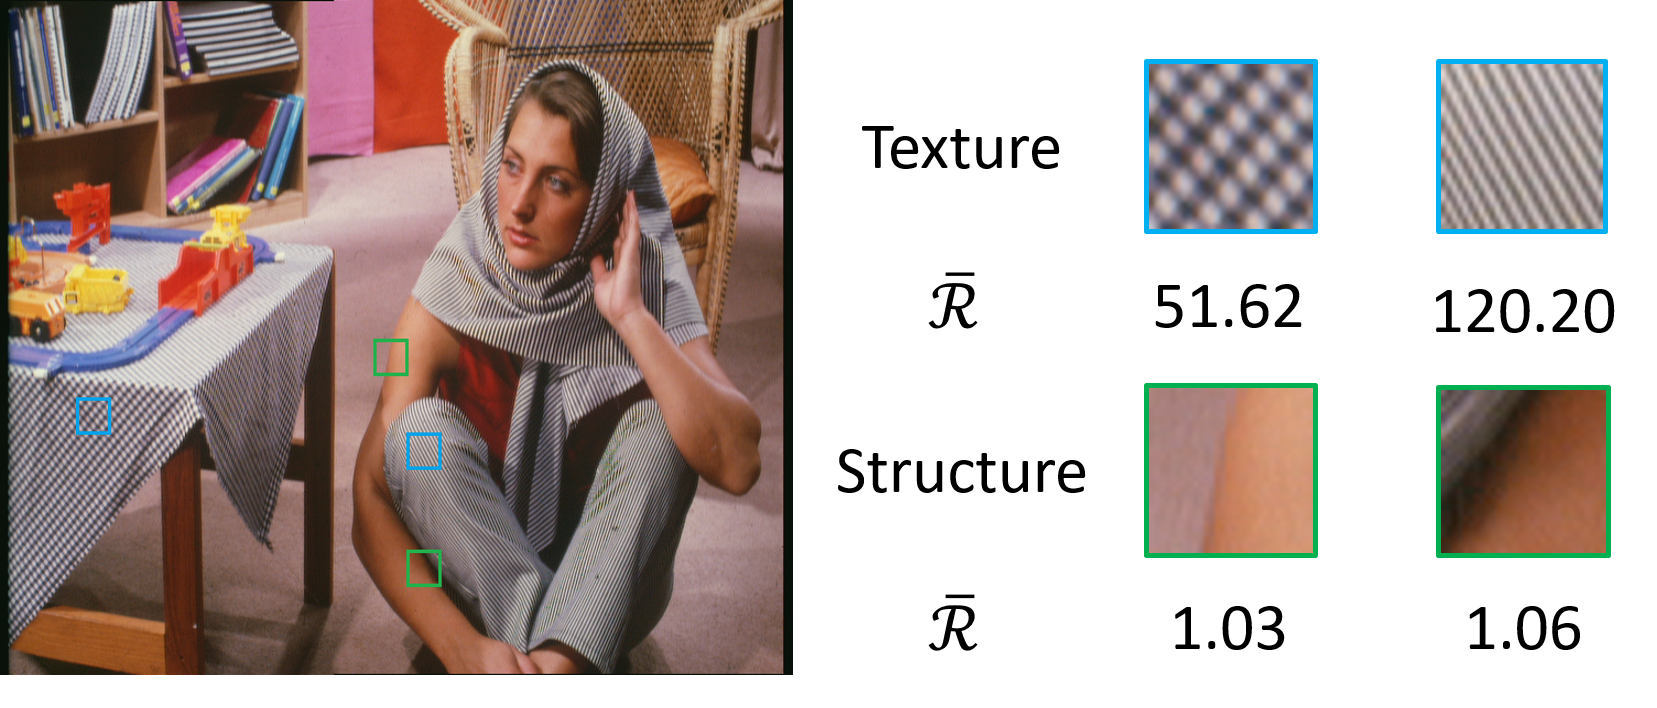
\includegraphics[width=0.8\hsize]{images/jiep/analysis/analysis.eps}
	\caption{The images represent local variation deviation for different patches. $\bar{\mathcal{R}}$ is the average of variation deviation in the local patches. The local variation deviation surprisingly distinguish textures (blue regions) and structures (green regions).
	} \label{fig:jiep/analysis}
\end{figure}

Thanks to the performance of the LVD, Cai replaced the constraint term on the illumination with the LVD on the illumination in the minimization optimization problem as following:
\begin{equation}
 E(I, R) = \argmin_{R, I} \|R \circ I - S\|_{2}^{2} + \alpha{\left \|\frac{\nabla{I}}{\frac{1}{\Omega}\Sigma_{\Omega}\nabla{I} + \epsilon} \right\|_{1}} + \beta{\|\nabla{R}\|_{1}} + \gamma{\|I - B\|_{2}^{2}}, \label{eq:jiep}
\end{equation}
where $\alpha$, $\beta$, $\gamma$ are three positive parameters and $B$ ($B = max_{\Omega}(max_{c \in \{r, g, b\}}S_{c})$) represents the bright channel prior (BCP) of an observed image $S$. As shown in Fig.\ref{fig:jiep/example}, the estimated illumination removes texture component while preserving the structure information. Thus, in the estimated reflectance, JieP significantly suppresses the awareness of halo effect along with edge regions. Moreover, more textures detail reveal in the estimated reflectance.

%----JiePの図---- %
\begin{figure}[t]
	\begin{minipage}[b]{0.5\hsize}
		\centering
		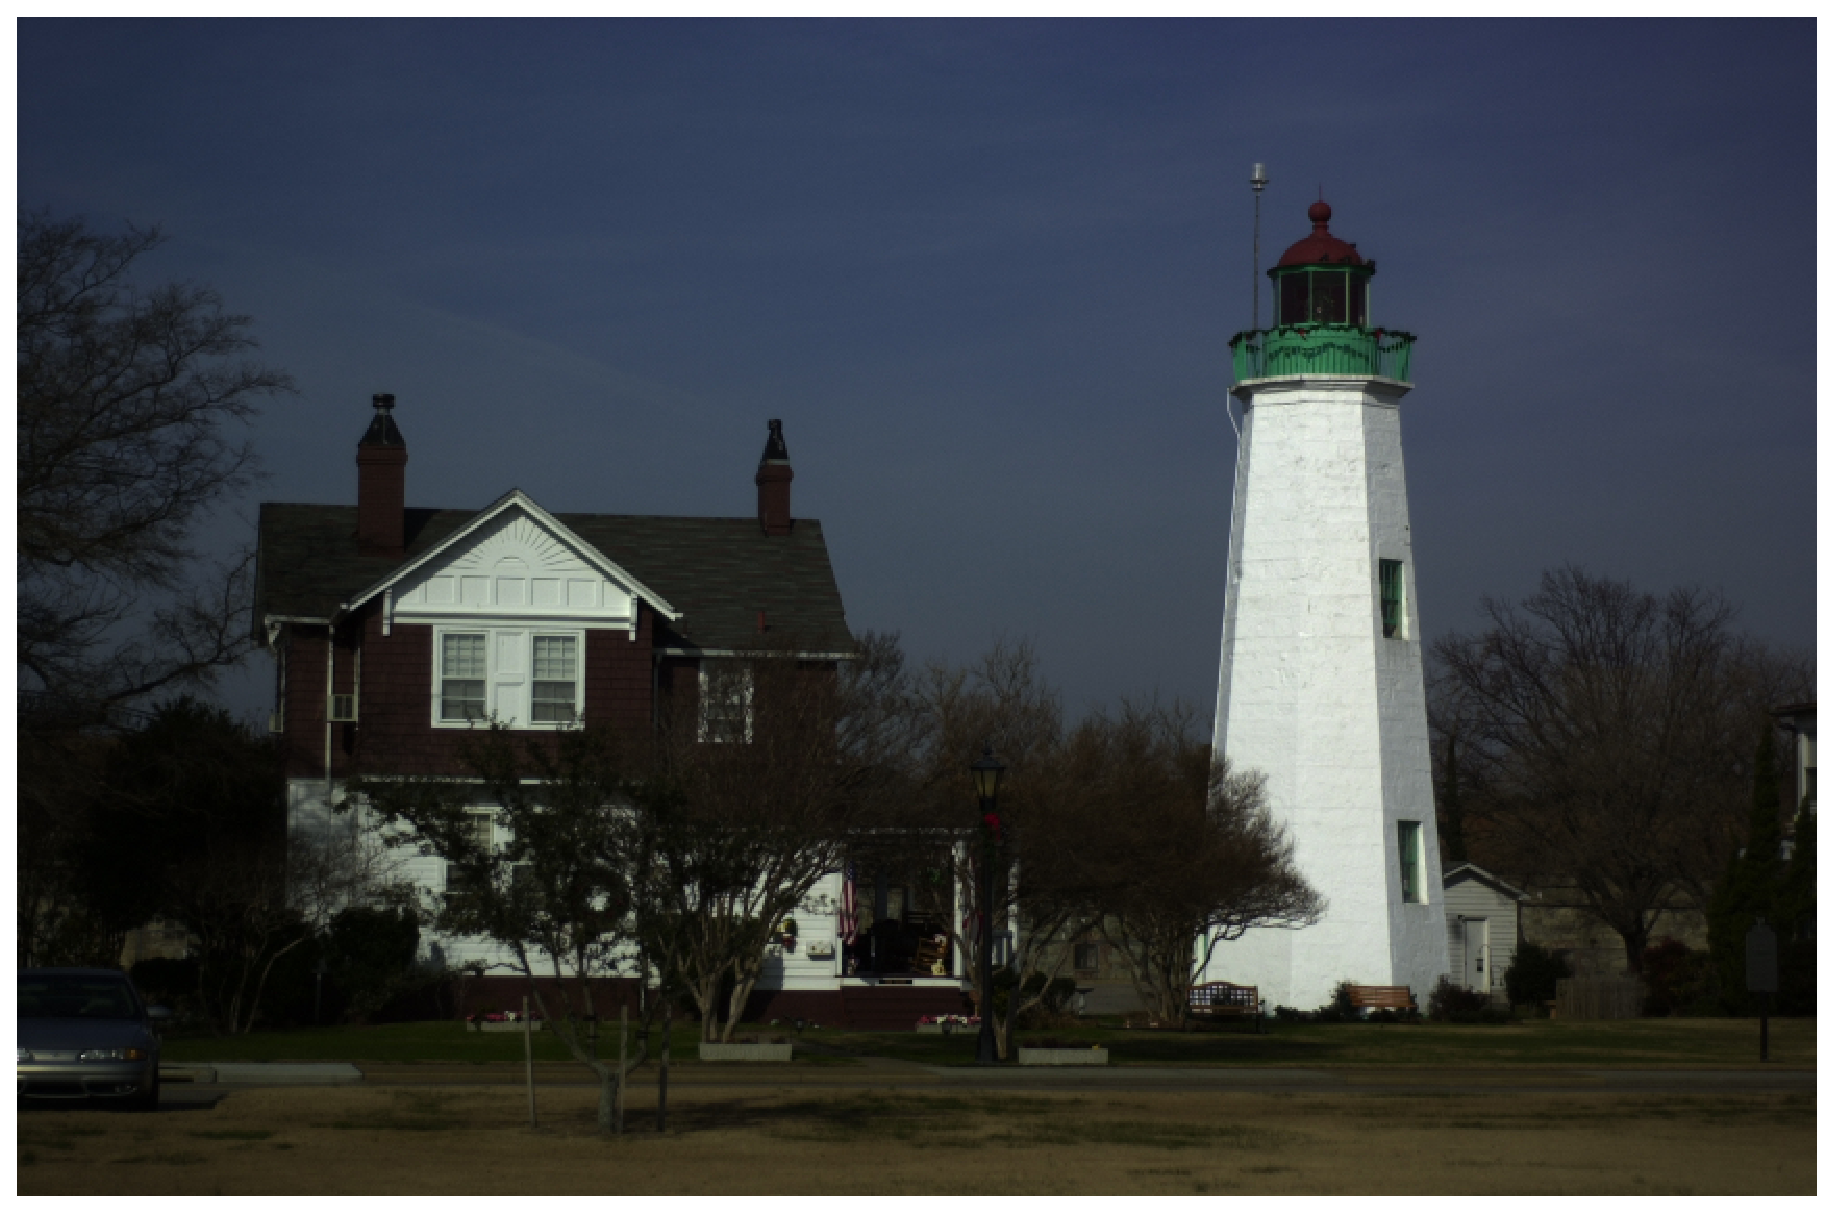
\includegraphics[width=62.5mm]{images/jiep/input.eps}
		\subcaption{Observed image $S$} \label{fig:jiep/input}
	\end{minipage}
	\begin{minipage}[b]{0.5\hsize}
		\centering
		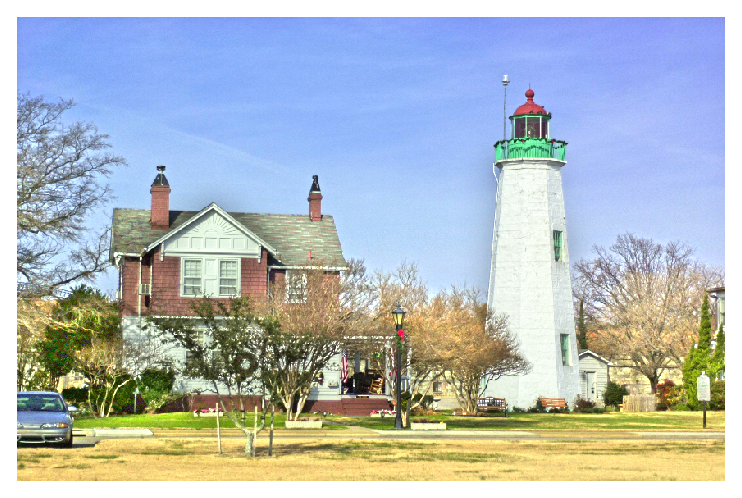
\includegraphics[width=62.5mm]{images/jiep/reflectance.eps}
		\subcaption{Reflectance $R$} \label{fig:jiep/reflectance}
	\end{minipage}
	\begin{minipage}[b]{0.5\hsize}
		\centering
		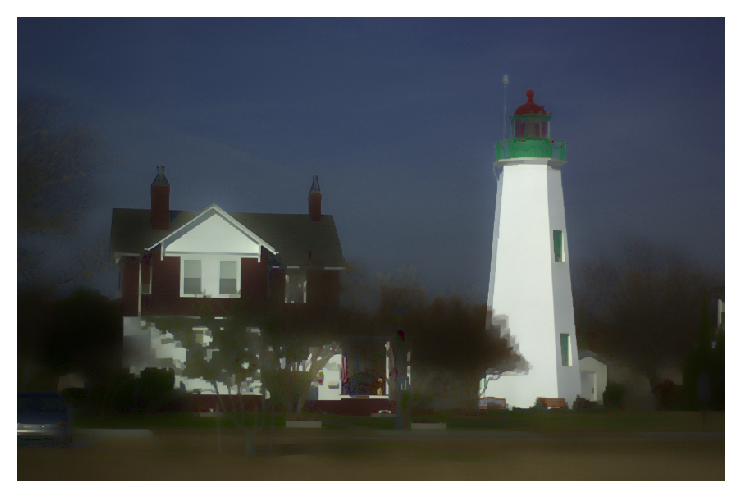
\includegraphics[width=62.5mm]{images/jiep/illumination.eps}
		\subcaption{Illumination $I$} \label{fig:jiep/illumination}
	\end{minipage}
	\begin{minipage}[b]{0.5\hsize}
		\centering
		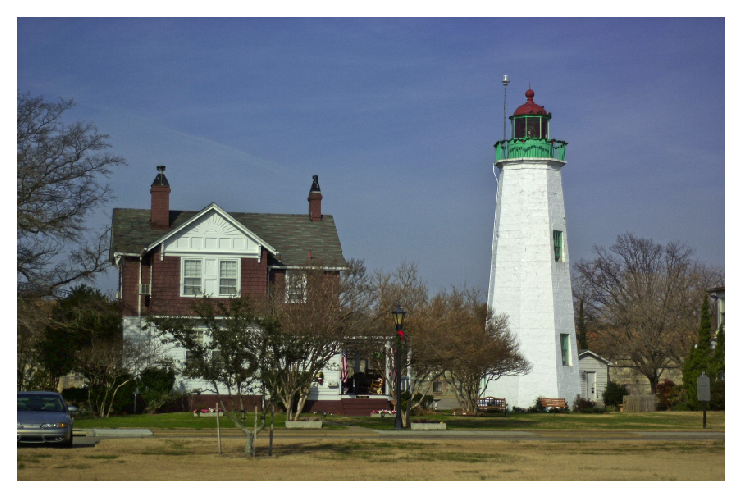
\includegraphics[width=62.5mm]{images/jiep/output.eps}
		\subcaption{Enhanced image $\hat{S}$} \label{fig:jiep/output}
	\end{minipage}
	\caption{The images represent the result of JieP \cite{jiep}.}
	\label{fig:jiep/example}
\end{figure}

\section{Consideration of Problems} \label{sec:problems}
These methods can enhance low-light images by solving each minimization optimization problem.
However, these methods have some problems in the enhanced image or the estimated component.
Therefore, in this section, the discussion centers on such problems with connected images.
\begin{itemize}
\item \textbf{SRIE.}
This method is prone to over-smooth the illumination component without preserving the structure information because of the constraint term $L_{2}$ that the illumination should be spatially smooth. 
As a result, as shown in Fig. \ref{fig:problem/srie/reflectance}, the estimated reflectance generates halo effect along with edge regions that have large intensity gradient. 
Moreover, as can be seen in Fig. \ref{fig:variational/reflectance}, in the estimated reflectance, much noise remain in dark regions and over-enhancement cause in bright regions because the constraint term on the reflectance is lack of the weight to distinguish between dark and bright regions.
\end{itemize}
\begin{itemize}
\item \textbf{JieP.}
This method can significantly take consideration of the constraint term on the illumination, but is not sufficient for the reflectance. Therefore, as can be seen in Fig. \ref{fig:problem/jiep/reflectance}, the estimated reflectance have much noise in dark regions and over-enhance in bright regions. Moreover, the constraint term on the illumination adopts L1 norm regularization, so that it may damage structure information too much in the estimated illumination.
\end{itemize}

%----Problemsの図---- %
\begin{figure}[t]
	\begin{minipage}[b]{1.0\hsize}
		\centering
		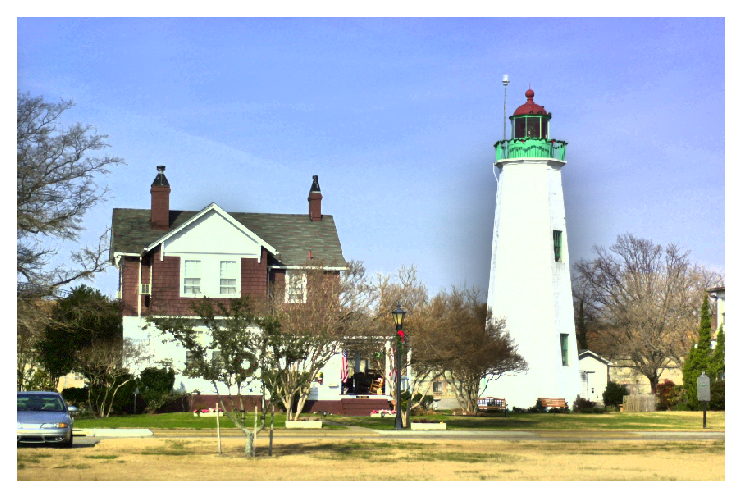
\includegraphics[width=0.65\hsize]{images/problems/srie/reflectance.eps}
		\subcaption{Reflectance (SRIE)} \label{fig:problem/srie/reflectance}
	\end{minipage}\\
	\begin{minipage}[b]{1.0\hsize}
		\centering
		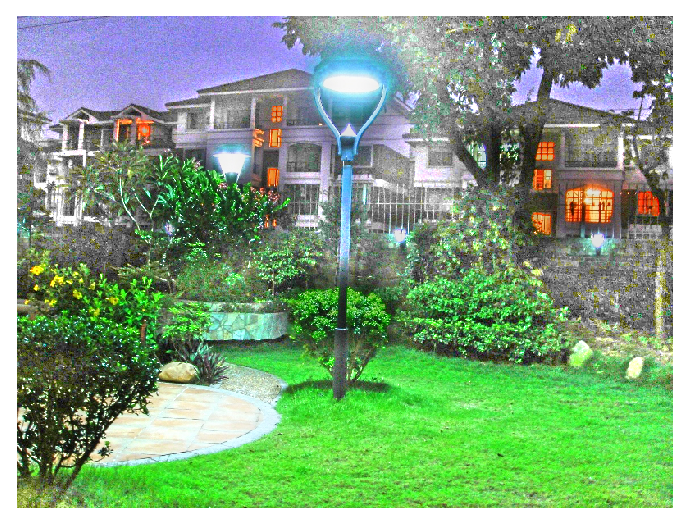
\includegraphics[width=0.65\hsize]{images/problems/jiep/reflectance.eps}
		\subcaption{Reflectance (JieP)} \label{fig:problem/jiep/reflectance}
	\end{minipage}
	\caption{The images represent each problem of these methods.}
	\label{fig:problems}
\end{figure}